Sikteeri on Kapsi ry:n laskutuksen ja jäsenhallinnan tarpeisiin kehitetty web-palvelu. Sikteeriin on pääsy Kapsi ry:n hallituksella, ylläpidolla ja ryhmään laskutus kuuluvilla jäsenillä. Lisäksi yhdistyksellä on käytössään erillinen komentorivityökalu, nimeltä admtool, jolla voidaan tehdä erilaisia ylläpitotehtäviä.

Sekä Sikteeri että admtool käyttävät ulkoisena komponenttina LDAP-käyttäjähallintaa, josta tarkistetaan onko käyttäjällä oikeuksia käyttää kyseisiä palveluita. Nykyinen arkkitehtuuri on kuvattu kuvassa \ref{kapsi_nykyinen}. Kuvaan on lisätty myös suunnitteilla oleva käyttäjien palvelunhallinta, jota kautta jäsenet voisivat lisätä itselleen jäsenmaksuun kuuluvia palveluita, kuten sähköpostialiaksia ja domaineja. Myös käyttäjien palvelunhallinnan tarvitsee tunnistaa käyttäjät, joten nykyisessä arkkitehtuurissa myös sen täytyy integroitua LDAP-käyttäjänhallintaan.

\begin{figure}[h]
\centering
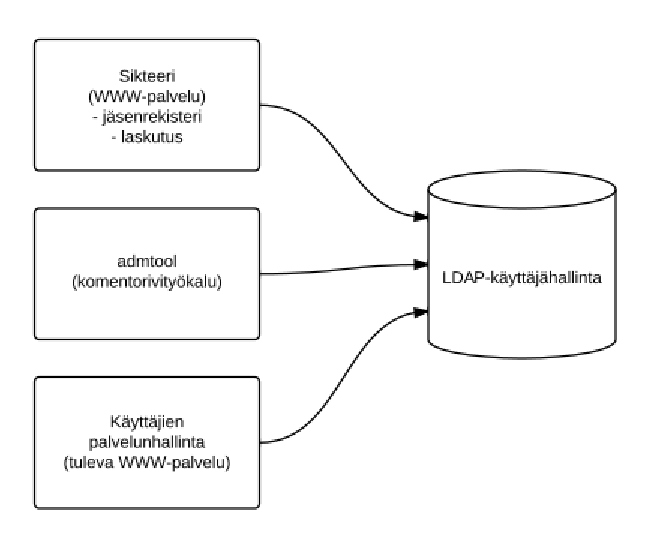
\includegraphics[width=.7\textwidth]{toteutus/kapsi_nykyinen.eps}
\caption{Kapsin jäsenhallintapalveluiden arkkitehtuuri.}%
\label{kapsi_nykyinen}
\end{figure}

\begin{figure}[ht]
\centering
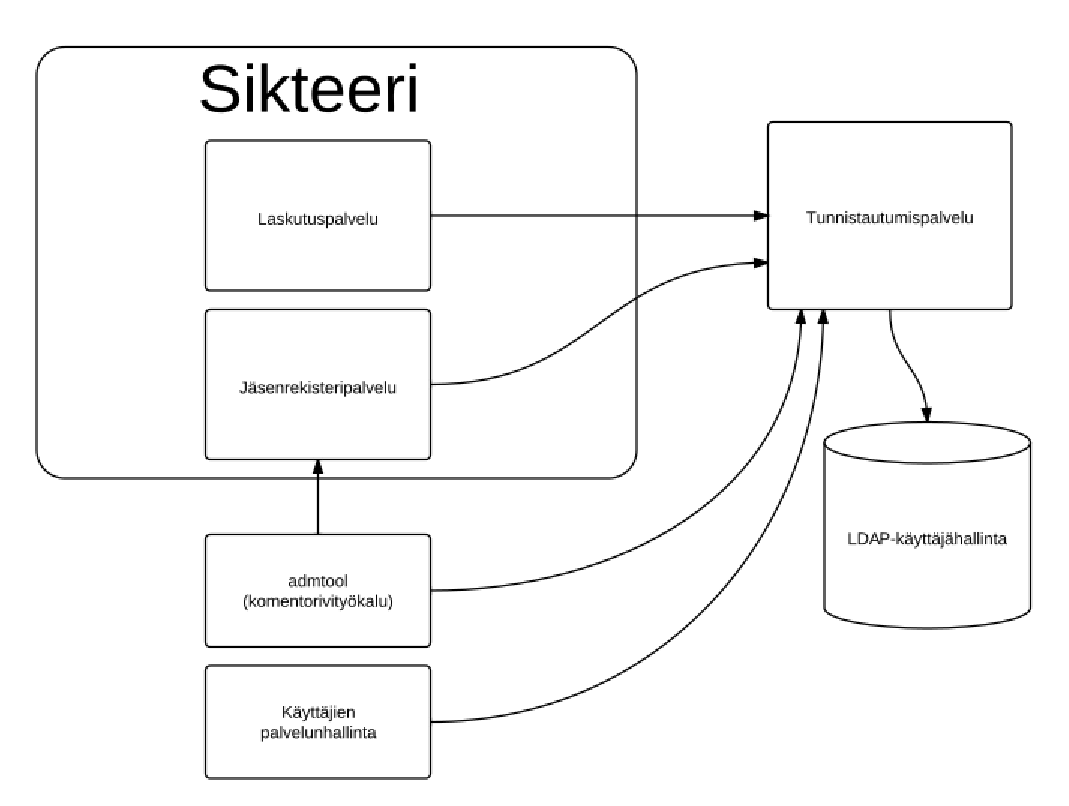
\includegraphics[width=.7\textwidth]{toteutus/kapsi_uusi.eps}
\caption{Palvelusuuntautuneen arkkitehtuurin mukainen kuvaus Kapsin järjestelmästä. Sikteerin palvelut on jaoteltu omiksi komponenteiksi ja järjestelmään on lisätty keskitetty tunnistautumispalvelu.}%
\label{kapsi_uusi}
\end{figure}


Giganttinen web-palvelin, joka hoitaa Kaiken tällä hetkellä.

LDAP, jossa käyttäjät, integroitu web-palveluihin.

halutaan olla SOA.

Sikteeri on Kapsin jäsenrekisteri ja laskutusohjelmisto. Tämä täytyisi selittää auki tekstissä, koska se on oleellisin juttu kokonaisuden kannalta.
